\documentclass[fleqn]{beamer}\usepackage[]{graphicx}\usepackage[]{color}
% maxwidth is the original width if it is less than linewidth
% otherwise use linewidth (to make sure the graphics do not exceed the margin)
\makeatletter
\def\maxwidth{ %
  \ifdim\Gin@nat@width>\linewidth
    \linewidth
  \else
    \Gin@nat@width
  \fi
}
\makeatother

\definecolor{fgcolor}{rgb}{0.345, 0.345, 0.345}
\makeatletter
\@ifundefined{AddToHook}{}{\AddToHook{package/xcolor/after}{\definecolor{fgcolor}{rgb}{0.345, 0.345, 0.345}}}
\makeatother
\newcommand{\hlnum}[1]{\textcolor[rgb]{0.686,0.059,0.569}{#1}}%
\newcommand{\hlstr}[1]{\textcolor[rgb]{0.192,0.494,0.8}{#1}}%
\newcommand{\hlcom}[1]{\textcolor[rgb]{0.678,0.584,0.686}{\textit{#1}}}%
\newcommand{\hlopt}[1]{\textcolor[rgb]{0,0,0}{#1}}%
\newcommand{\hlstd}[1]{\textcolor[rgb]{0.345,0.345,0.345}{#1}}%
\newcommand{\hlkwa}[1]{\textcolor[rgb]{0.161,0.373,0.58}{\textbf{#1}}}%
\newcommand{\hlkwb}[1]{\textcolor[rgb]{0.69,0.353,0.396}{#1}}%
\newcommand{\hlkwc}[1]{\textcolor[rgb]{0.333,0.667,0.333}{#1}}%
\newcommand{\hlkwd}[1]{\textcolor[rgb]{0.737,0.353,0.396}{\textbf{#1}}}%
\let\hlipl\hlkwb

\usepackage{framed}
\makeatletter
\newenvironment{kframe}{%
 \def\at@end@of@kframe{}%
 \ifinner\ifhmode%
  \def\at@end@of@kframe{\end{minipage}}%
  \begin{minipage}{\columnwidth}%
 \fi\fi%
 \def\FrameCommand##1{\hskip\@totalleftmargin \hskip-\fboxsep
 \colorbox{shadecolor}{##1}\hskip-\fboxsep
     % There is no \\@totalrightmargin, so:
     \hskip-\linewidth \hskip-\@totalleftmargin \hskip\columnwidth}%
 \MakeFramed {\advance\hsize-\width
   \@totalleftmargin\z@ \linewidth\hsize
   \@setminipage}}%
 {\par\unskip\endMakeFramed%
 \at@end@of@kframe}
\makeatother

\definecolor{shadecolor}{rgb}{.97, .97, .97}
\definecolor{messagecolor}{rgb}{0, 0, 0}
\definecolor{warningcolor}{rgb}{1, 0, 1}
\definecolor{errorcolor}{rgb}{1, 0, 0}
\makeatletter
\@ifundefined{AddToHook}{}{\AddToHook{package/xcolor/after}{
\definecolor{shadecolor}{rgb}{.97, .97, .97}
\definecolor{messagecolor}{rgb}{0, 0, 0}
\definecolor{warningcolor}{rgb}{1, 0, 1}
\definecolor{errorcolor}{rgb}{1, 0, 0}
}}
\makeatother
\newenvironment{knitrout}{}{} % an empty environment to be redefined in TeX

\usepackage{alltt}
\usepackage[english]{babel}

\usepackage{amsmath,amssymb}
\usepackage{graphicx}

% vertical separator macro
\newcommand{\vsep}{
  \column{0.0\textwidth}
    \begin{tikzpicture}
      \draw[very thick,black!10] (0,0) -- (0,7.3);
    \end{tikzpicture}
}

% More space between lines in align
\setlength{\mathindent}{0pt}

% Beamer theme
\usetheme{ZMBZFMK}
\usefonttheme[onlysmall]{structurebold}
\mode<presentation>
%\setbeamercovered{transparent=10}

% align spacing
\setlength{\jot}{0pt}


\AtBeginSection[]
{
  \begin{frame}
    \frametitle{Table of Contents}
    \tableofcontents[currentsection]
  \end{frame}
}
\AtBeginSubsection[]
{
  \begin{frame}
    \frametitle{Table of Contents}
    \tableofcontents[currentsubsection]
  \end{frame}
}


% Only the first Slide
\title{Reproducible research: with R, renv and \LaTeX}
\author{Liberty Mlambo}
\institute[SB Stats Group]{ Research Assistant:\\ University of Nottingham}
\date{\today}


% Make title page
\IfFileExists{upquote.sty}{\usepackage{upquote}}{}
\begin{document}
\begin{frame}
  \titlepage
\end{frame}

% Índice
\begin{frame}{Table of Contents}
    \tableofcontents
\end{frame}

% Frame 1
\section{Background}
\begin{frame}
  \frametitle{Requirements}
    We will talk about the following software:
    \begin{itemize}[<+->]
      \item R 
      \item RStudio
      \item \LaTeX
      \item tinytex
      \item renv
      \item knitr (preinstalled with RStudio)
      \item R package installation access
      \item Overleaf
    \end{itemize}
\end{frame}

\section{¿Cómo funciona?}
\subsection{Intuición en general}
\begin{frame}{Curvas de Nivel}
    \begin{itemize}
        \item Conjunto de Nivel: $\ell_{f}(\vec{x}_0)= \{\vec{x}: f(\vec{x}) = f(\vec{x}_0) \}$
        \item Curva de Nivel: Una parte conexa de $\ell_f(\vec{x}_0)$
    \end{itemize}
\end{frame}

% \begin{frame}{Primera Curva de Nivel}
%     \begin{figure}
%         \centering
%         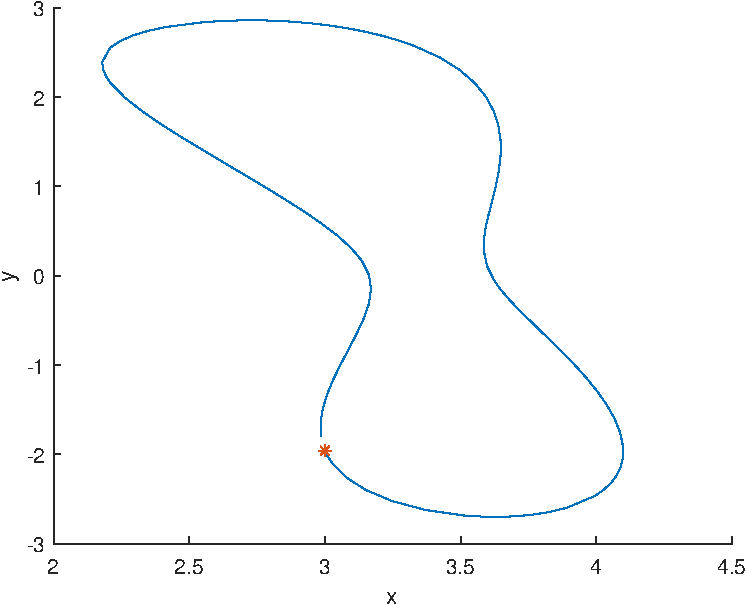
\includegraphics[width = 0.6\textwidth]{Hourglass-cropped.pdf}
%         \caption{Función de Himmelblau: $\vec{x}_0 = (3,-2)$}
%         \label{fig:my_label}
%     \end{figure}
% \end{frame}
% 
% \begin{frame}{Encontrando Mínimos}
%     \begin{figure}
%         \centering
%         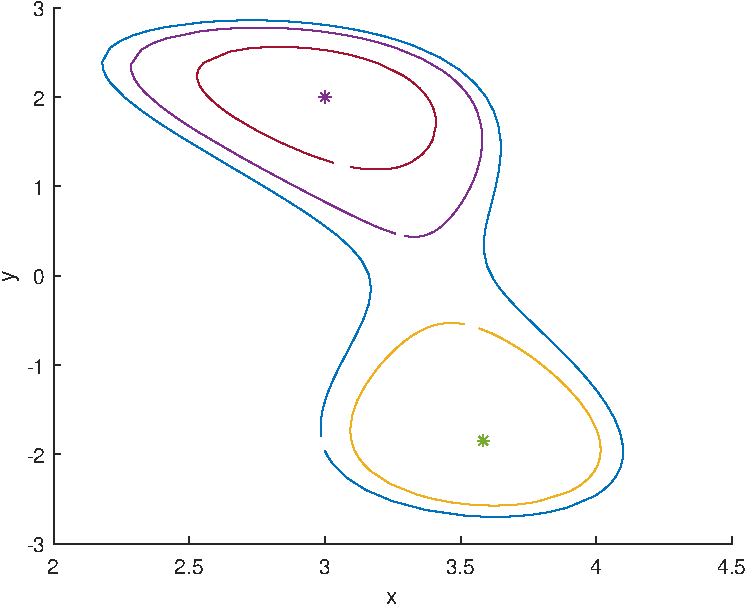
\includegraphics[width = 0.6\textwidth]{FirstSplit-cropped.pdf}
%         \caption{Función de Himmelblau: $\vec{x}_0 = (3,-2)$}
%         \label{fig:my_label}
%     \end{figure}
% \end{frame}
% 
% \begin{frame}
%   \frametitle{Haz recursión y conquistarás...}
%   \begin{figure}
%       \centering
%       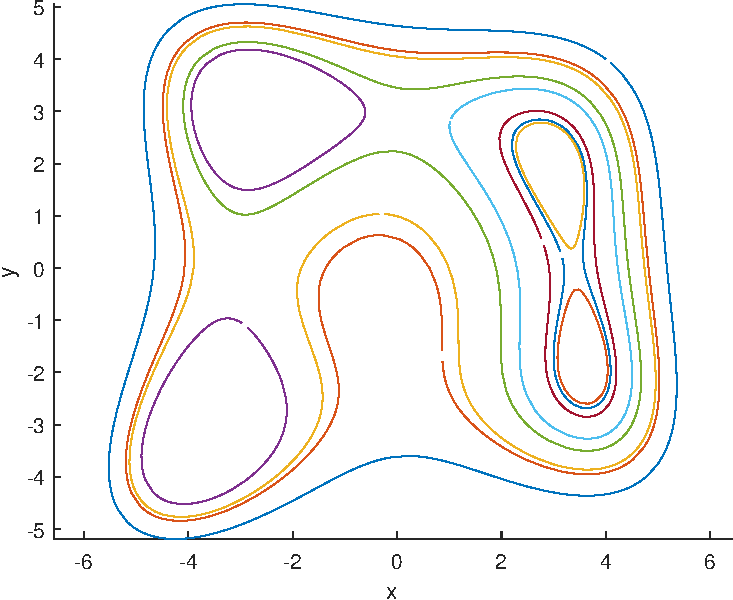
\includegraphics[width = 0.6\textwidth]{FullMethod.pdf}
%       \caption{Función de Himmelblau: $\vec{x}_0 = (4,4)$}
%       \label{fig:my_label}
%   \end{figure}
% \end{frame}
% 
% 
% \subsection{Siguiendo curvas de nivel}
% \begin{frame}
%     \frametitle{Para Seguir una Curva de Nivel}
%     \begin{block}{Requisitos:}
%         Introducir un parámetro de tiempo, $t$. Así, $\Phi(t) = (x(t),y(t))$ es la parametrización de la curva de nivel.\\
%         \vspace{10 pt}
%         Encontrar una EDO que siga la curva. \\
%         \vspace{10 pt}
%         Aplicar un método numérico que siga la EDO
%     \end{block}
% \end{frame}
% 
% \begin{frame}{Obteniendo una EDO}
%     Sabemos que $\nabla f(\vec{x})$ y la curva de nivel son perpendiculares.\\
%     \vspace{10 pt}
%     Calculamos $\nabla f(\vec{x})$ de manera exacta o con diferencias finitas.\\
%    \vspace{ 10pt}
%    Multiplicamos por $A = \begin{pmatrix}
%    0 & -1 \\
%    1 & 0
%    \end{pmatrix}$ para girar $90^{\circ}$\\
%    \vspace{ 10pt}
%     Así, $\begin{pmatrix}
%     \dot{x} \\
%     \dot{y}
%     \end{pmatrix}
%     =
%     \begin{pmatrix}
%    0 & -1 \\
%    1 & 0
%    \end{pmatrix} \nabla f(\vec{x})$, es la EDO que necesitamos para seguir la curva de nivel.
% \end{frame}
% 
% \begin{frame}{La EDO}
%    Definimos $H(x) = \begin{pmatrix}
%    0 & -1 \\
%    1 & 0
%    \end{pmatrix} \nabla f(\vec{x})$, y tenemos el siguiente PVI:\\
%    \vspace{10 pt}
%    \begin{block}{PVI en cada paso:}
%    $$\begin{pmatrix}
%     \dot{x} \\
%     \dot{y}
%     \end{pmatrix}
%     =
%     \frac{H(\vec{x})}{\max\{1,\left|| \nabla f(\vec{x}(t_i))\right||\}}$$\\
%     \vspace{3 pt}
%     $$\vec{x}(0) = \vec{x}(t_i)$$
%    \end{block}
% \end{frame}
% 
% \begin{frame}{¿Cómo seguir esa EDO?}
%     \begin{itemize}
%         \item RK4
%         \item Trapecio Explícito
%         \item ¡Muchos más!
%     \end{itemize}
% \end{frame}
% 
% 
% 
% \subsection{Decidiendo qué hacer}
% 
% \begin{frame}{Una Medida Importante}
%     \begin{block}{Para medir la curvatura...}
%         $\theta_i$ es el ángulo de $\nabla f(\vec{x}_i)$ respecto al eje $x$. 
%     \end{block}
%     \begin{figure}
%     \centering
%     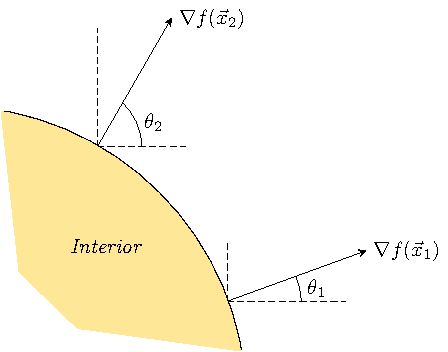
\includegraphics[width = 0.5\textwidth]{figure31.pdf}
%     \caption{Midiendo la Curvatura}
%     \label{fig:my_label}
% \end{figure}
% \end{frame}
% 
% \begin{frame}{Convexidad y Concavidad}
%     \begin{block}{Tres opciones:}
%         \begin{itemize}[<+->]
%             \item Donde $\theta^{'} > 0$, la curva de nivel es convexa (bien inflada).
%             \item Donde $\theta^{'} < 0$, la curva de nivel es cóncava (hundida hacia adentro).
%             \item Donde $\theta^{'} = 0$, la curva de nivel es una línea recta. 
%         \end{itemize}
%     \end{block}
% \end{frame}
% 
% \begin{frame}{Ejemplo Ilustrativo}
%     \begin{columns}
%     \column{0.5\textwidth}
%         \begin{figure}
%             \centering
%             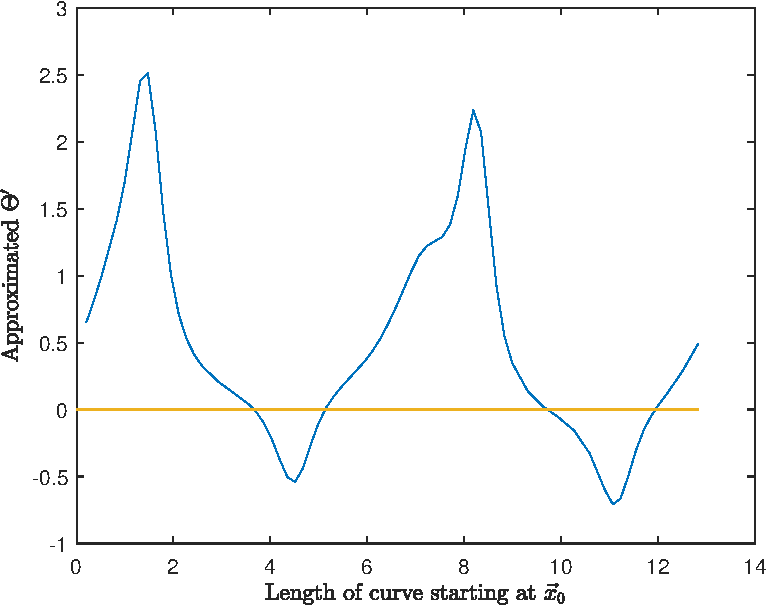
\includegraphics[width = \textwidth]{FINALIHOPE-cropped.pdf}
%             \label{fig:my_label}
%         \end{figure}
%     \column{0.5\textwidth}
%         \begin{figure}
%             \centering
%             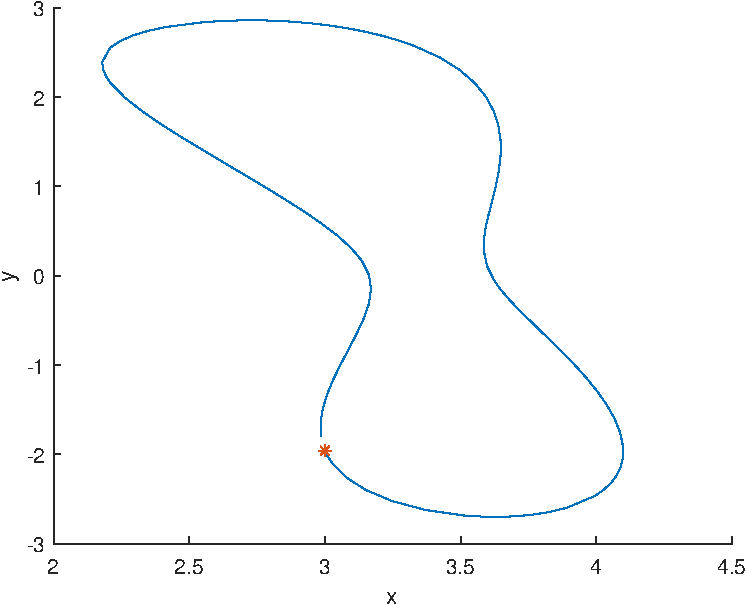
\includegraphics[width = \textwidth]{Hourglass-cropped.pdf}
%             \label{dual}
%         \end{figure}
%     \end{columns}
%     \centering{Figura: Una Curva de Nivel y su medida $\theta^{'}$}
% \end{frame}
% 
% \begin{frame}{Recursión por Ruptura}
% \begin{block}{Def: Picos negativos}
%     Para una curva de nivel $M_{\vec{x}_0}$, los \emph{Picos Negativos} son aquellos puntos $\vec{x}_i$ donde $\theta^{'}_i$ alcanza un mínimo
% \end{block}
%     Si dos Picos Negativos están cerca, creamos una \emph{ruptura}. %Es decir, tomamos $\vec{y}_0$ y $\vec{z}_0$ en lados opuestos de los Picos Negativos, y llamamos recursivamente al método sobre $\vec{y}_0$ y $\vec{z}_0$.
% \end{frame}
% 
% \begin{frame}{Recursión por Ruptura}
%     \begin{figure}
%         \centering
%         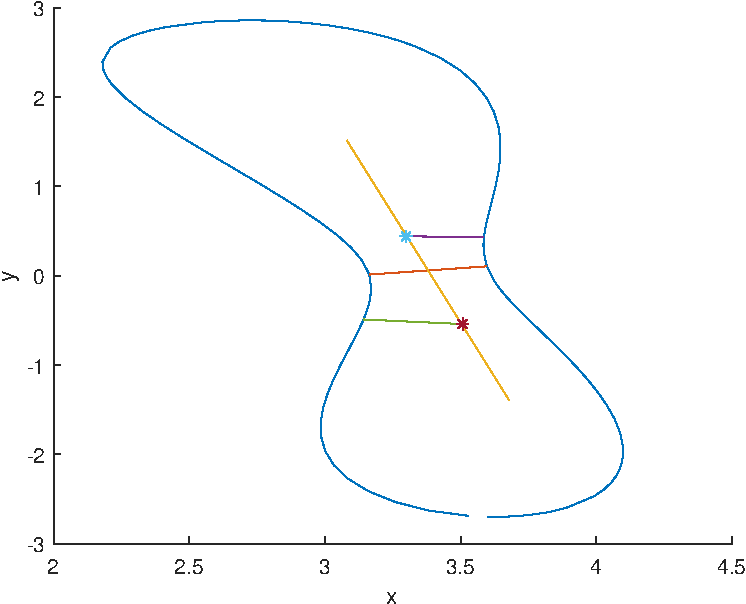
\includegraphics[width = 0.6\textwidth]{SiSePudo-cropped.pdf}
%         \caption{Ruptura}
%         \label{fig:my_label}
%     \end{figure}
% \end{frame}
% 
% \begin{frame}{Encontrar el Mínimo}
%     \begin{block}{Convexidad Global}
%         Si $\theta^{'}_i>0$ para toda $i$, entonces la curva de nivel es \emph{globalmente convexa.}
%     \end{block}
%     \vspace{10 pt}
%         Si una curva de nivel es globalmente convexa, entonces:\\
%         \vspace{10 pt}
%         \begin{columns}
%         \column{0.4\textwidth}
%         \begin{block}{¿Está cerca de un mínimo?}
%           Método de Newton
%         \end{block}
%         \column{0.4\textwidth}
%         \begin{block}{¿Está lejos?}
%          Bajar el Nivel
%         \end{block}
%         \end{columns}
% \end{frame}
% 
% \begin{frame}{Bajar el Nivel}
%         Sea $L$ la longitud de la curva. Luego, tomamos:\\  $$\vec{y}_0 = \vec{x}_i-kL\frac{\nabla f(\vec{x})}{\left||\nabla f(\vec{x})\right||}$$ 
%         \vspace{10 pt} 
%         Aquí, $k$ es un parámetro que representa la proporción de $L$ a avanzar. 
% \end{frame}
% 
% \begin{frame}{Bajar el Nivel}
%     \begin{figure}
%         \centering
%         
\includegraphics[width = \textwidth]{Logo.png}
%         %\caption{Bajando el Nivel sin Convexidad Global}
%         \label{fig:my_label}
%     \end{figure}
% \end{frame}
% 
% 
% \begin{frame}{Esquema General}
%     \begin{figure}
%         \centering
%         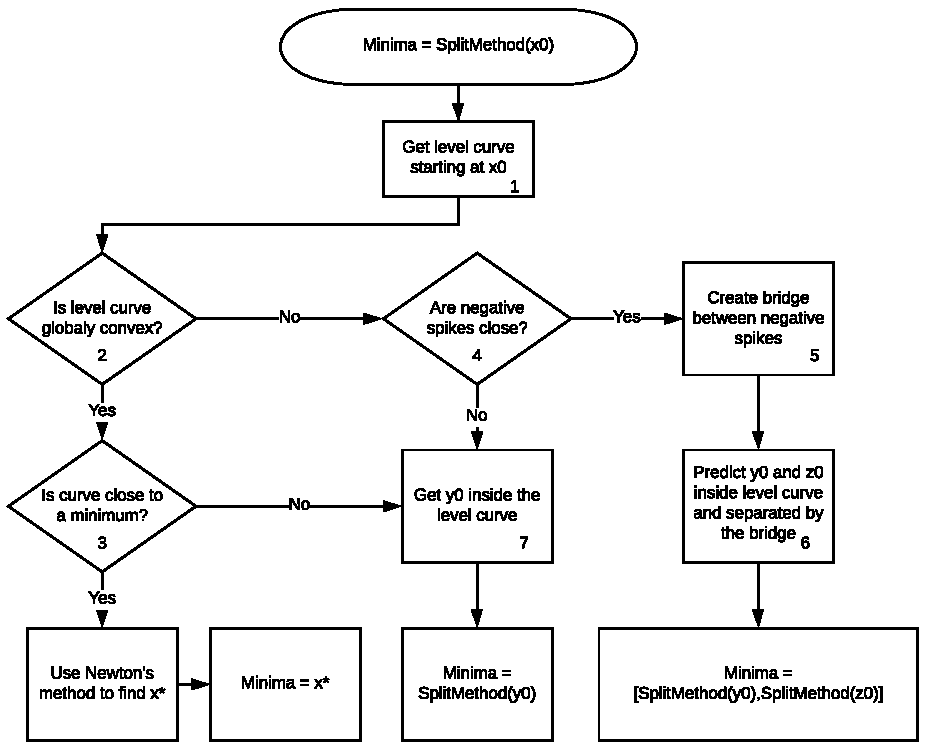
\includegraphics[width = 0.75\textwidth]{SplitMethod.pdf}
%  %       \caption{Método Completo}
%         \label{fig:my_label}
%     \end{figure}
% \end{frame}
% 
% \section{Resultados y comentarios}
% \begin{frame}{Resultados}
%     \begin{table}[h]
%     \centering
%     \caption{Función de Himmelblau: $\vec{x}_0 = (4,4)$}
%     \begin{tabular}{|c|c|c|}\hline 
%     Minimos & Minimos estimados & Error  \\
%     \hline
%     (3.0,2.0) & (3.0000..., 1.9999...) & 1.7117 e-12\\
%     (-2.805118, 3.131312) & (-2.805118..., 3.131312...) & 5.3283 e-07\\
%     (-3.779310, -3.283186) & (-3.779310..., -3.283185...) &  2.5449 e-07\\
%     (3.584428, -1.848126) & (3.584428..., -1.848126...) & 6.2730 e-07\\
%     \hline 
%     \end{tabular}
%     \label{tab:HimMinima}
% \end{table}
% \end{frame}
% 
% \begin{frame}{Resultados}
% \begin{table}[h]
%     \centering
%     \caption{Método de la ruptura aplicado a diferentes funciones}
%     \begin{tabular}{|c|c|c|c|}\hline
%     Función & $\vec{x}_0$ & Minimos estimados & Error \\
%     \hline 
%     Styblinski -Tang    & (4,4) &(-2.9035,-2.9035) & 3.9274e-08\\
%     Easom  &  (1.6,1.6) &(3.1415,3.1415) & 1.7796e-11\\
%     Booth  & (0,10) &(0.9999,2.9999) & 1.0422e-09\\
%     White \& Holst     & (0,0) &(0.9999,0.9999) & 4.2564e-11\\
%     \hline
%     \end{tabular}
%     \label{tab:Various}
% \end{table}
% \end{frame}
% 
% 
% \begin{frame}{Comentarios}
%     \begin{itemize}[<+->]
%         \item El método requiere funciones suaves y con curvas de nivel cerradas.
%         \item Aproxima bien los mínimos, aunque algunos parámetros deben ser ajustados para cada función $f$.
%         \item Tener información parcial sobre el conjunto de nivel ha sido un problema constante.
%     \end{itemize}
% \end{frame}
% 
% \begin{frame}{Bibliografía}
% \begin{enumerate}
%     \item Amir Beck, \emph{Introduction to Nonlinear Optimization - Theory, Algorithms and Applications} MOS-SIAM series on Optimization. SIAM, 2014.\\
%     \item Andrei Neculai, \emph{An Unconstrained Optimization Test Function Collection} Advanced Modeling and Optimization, Vol. 10, number 1, 2008.\\
%     \item Jorge Nocedal and Stephen Wright,  \emph{Numerical Optimization}. New York: Springer, 2006.
% \end{enumerate}
% \end{frame}

\end{document}
